\begin{enumerate}[label=\thesubsection.\arabic*,ref=\thesubsection.\theenumi]
	\item Find the values of $\theta \text{ and } p$, if the equation $x\cos\theta+y\sin\theta=p$ is the normal form
of the line $\sqrt{3}x+y+2=0$.
\\
\solution
				\begin{align}
	\vec{n}=\myvec{\sqrt{3}\\1},
			c=-2
			\\
			\implies
			\theta=\tan^{-1}\brak{\sqrt{3}}
			=\frac{\pi}{3},
			p=\frac{\abs{c}}{\norm{\vec{n}}}=1
		\end{align}
See \figref{fig:chapters/11/10/4/2/Fig1}.
\begin{figure}[H]
	\begin{center} 
	    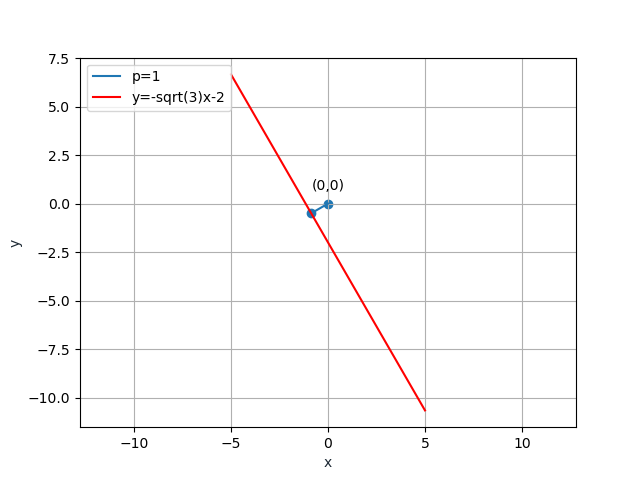
\includegraphics[width=0.75\columnwidth]{chapters/11/10/4/2/figs/line.png}
	\end{center}
\caption{}
\label{fig:chapters/11/10/4/2/Fig1}
\end{figure}


\item  Reduce the following equations into normal form. Find their perpendicular distances from the origin and angle between perpendicular and the positive $x$-axis.
\label{chapters/11/10/3/3}
\begin{enumerate}
	\item $x-\sqrt{3}y+8=0$ 
	\item $y-2=0$
	\item $x-y=4$
\end{enumerate}
\solution
\iffalse
\documentclass[12pt]{article}
\usepackage{graphicx}
\usepackage{amsmath}
\usepackage{mathtools}
\usepackage{gensymb}
\usepackage[utf8]{inputenc}
\usepackage{float}
\newcommand{\mydet}[1]{\ensuremath{\begin{vmatrix}#1\end{vmatrix}}}
\providecommand{\brak}[1]{\ensuremath{\left(#1\right)}}
\providecommand{\norm}[1]{\left\lVert#1\right\rVert}
\newcommand{\solution}{\noindent \textbf{Solution: }}
\newcommand{\myvec}[1]{\ensuremath{\begin{pmatrix}#1\end{pmatrix}}}
\let\vec\mathbf

\begin{document}
\begin{center}
\textbf\large{CLASS-11 \\ CHAPTER-10 \\ STRAIGHT LINES}
\end{center}
\section*{Excercise 10.3}

\solution
\fi
\begin{enumerate}
\item The given equation can be expressed as
		\begin{align}
			\myvec{ 1 & -\sqrt{3}}\vec{x}= -8
			\end{align}
			yielding
\begin{align}
			\vec{n} = \myvec{ 1 & -\sqrt{3}}, c = -8
\end{align}
From the above, the	angle between perpendicular and the positive $x$-axis is given by
		\begin{align}
			\tan^{-1}\brak{-\sqrt{3}} = \frac{2\pi}{3}
		\end{align}
	The perpendicular distance from the origin to the line is given by
		\begin{align}
			d=\frac{\abs{c}}{\norm{\vec{n}}}=4
		\end{align}
\item In this case, the given equation becomes
          \begin{align}
		  \myvec{0 & 1}\vec{x} = 2
          \end{align}
	  yielding
                  \begin{align}
			  \vec{n}=\myvec{0\\1}, c = 2
                          \end{align}
          Angle between perpendicular and the positive $x$-axis is given by:
		\begin{align}  
			\tan^{-1}\infty = \frac{\pi}{2}
                \end{align}      
and  the perpendicular distance from the origin to the line is given by    
                                      \begin{align}
					      d=\frac{|c|}{\norm{\vec{n}}}=2             
                  \end{align}
\item   The given equation can be expressed as
                  \begin{align}
      \myvec{-1 & 1}\vec{x} = 4
                          \end{align}
			  yielding
                  \begin{align}
			  \vec{n}=\myvec{1\\-1}, c = 4
                          \end{align}
          Angle between perpendicular and the positive $x$-axis is given by
		\begin{align}   
			\tan^{-1}\brak{-1} = \frac{3\pi}{4}
                \end{align}                                                                           The perpendicular distance from the origin to the line is given by
		\begin{align}
			d=\frac{|c|}{\norm{\vec{n}}}=\frac{4}{\sqrt{2}}=2\sqrt{2}                    
                  \end{align}
\end{enumerate}
 

 \item  In each of the following cases, determine the direction cosines of the normal to
the plane and the distance from the origin.
\begin{enumerate}
	\item $z=2$ 
	\item $x + y + z = 1$
	\item $2x + 3y – z = 5$
	\item $5y + 8 = 0$
\end{enumerate}
    \solution
		  See 
  \tabref{tab:12/11/3/1}.
			\eqref{eq:PQ-final} was used for computing the distance from the origin.
			\begin{table}[H]
  \centering
  \begin{tabular}{|c|c|c|c|}
    \hline
    & $\vec{n}$ & $c$ & Distance \\
    \hline
    a) &		\myvec{0\\0\\1}  &2  & 2 \\
    \hline
    b) & $\myvec{1\\1\\1}$ & 1 & $\frac{1}{\sqrt{3}}$ \\
    \hline
    c) & $\myvec{2\\3\\-1}$ & 5 & $\frac{5}{\sqrt{14}}$ \\
    \hline
    d) & $\myvec{0\\-5\\0}$ & 8 & $\frac{8}{5}$ \\
    \hline
  \end{tabular}
  \caption{}
  \label{tab:12/11/3/1}
\end{table}
 


\item Find the distance of the point $(-1,1)$ from the line $12\brak{x+6} = 5\brak{y-2}$. 
\label{chapters/11/10/3/4}
	\\
\solution 
\begin{align}
		\vec{n} = \myvec{
	  12 \\
	  -5 
	  } ,   c = -82 
	  \\
	  \implies 
	d 
	= \frac{\abs{  \myvec{12 & -5 }\myvec{-1 \\ 1}-\brak{-82} }}{\sqrt{12^2+\brak{-5}^2}} 	
	= 5
\end{align}
\iffalse
See \figref{fig:11/10/3/4/Fig1}.
\begin{figure}[H]
	\begin{center}
		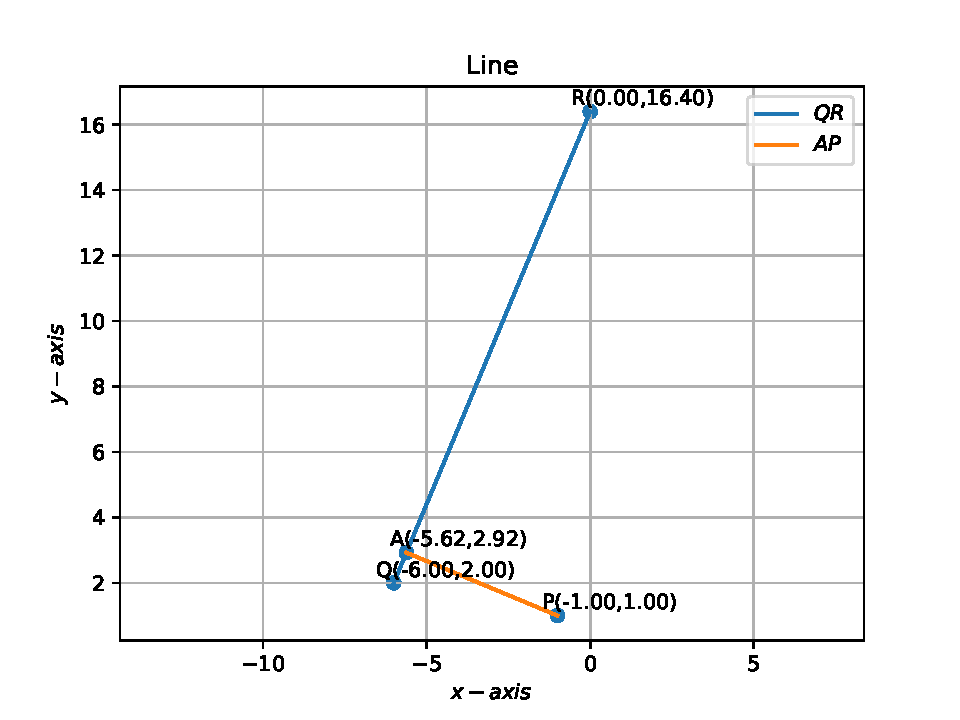
\includegraphics[width=0.75\columnwidth]{chapters/11/10/3/4/figs/problem4.pdf}
	\end{center}
\caption{}
\label{fig:11/10/3/4/Fig1}
\end{figure}
\fi

\item Find the coordinates of the foot of the perpendicular from $(-1, 3)$ to the line $3x-4y-16=0$.  
\label{chapters/11/10/3/14}
\\
\solution
Substituting
\begin{align}
 \vec{P}=\myvec{
-1\\
3
},
\vec{n}=\myvec{
3\\
-4
}, c=16
\end{align}
in 
	\eqref{eq:11/10/3/4/foot_of_perpendicular},
the desired foot of the perpendicular is then given by 
\begin{align}
\myvec{4&3\\3&-4}\vec{Q}=\myvec{\myvec{4&3}\myvec{-1\\3}\\16}
=\myvec{5\\16}  
\\
\implies
  \myvec{
   4 &  3  & 5\\
   3 & -4  & 16} 
  \xleftrightarrow[]{R_2=R_2-\frac{3}{4}R_1}
  \myvec{
  4 & 3 & 5\\
  0 & \frac{-25}{4} & \frac{49}{4}} 
\\
  \xleftrightarrow{R_2=\frac{-4}{25}}
  \myvec{
  4 & 3 & 5\\
  0 & 1 & \frac{-49}{25}}
  \xleftrightarrow{R_1=\frac{1}{4}R_1}
  \myvec{
  1 & \frac{3}{4} & \frac{5}{4}\\
  0 & 1 & \frac{-49}{25}}
\\
  \xleftrightarrow{R_1=R_1-\frac{3}{4}R_2}
  \myvec{
  1 & 0 & \frac{68}{25}\\
  0 & 1 & \frac{-49}{25}}          
\implies \vec{Q}=\myvec{
\frac{68}{25}\\[1pt]
\frac{-49}{25}
}
\end{align}
See 
\figref{fig:chapters/11/10/3/14/Fig}.
\begin{figure}[H]
	\begin{center} 
	    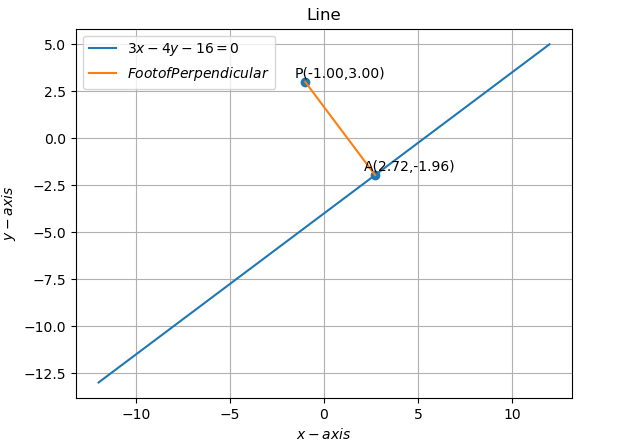
\includegraphics[width=0.75\columnwidth]{chapters/11/10/3/14/figs/lines.png}
	\end{center}
\caption{}
\label{fig:chapters/11/10/3/14/Fig}
\end{figure}

\item  If ${p}$ and ${q}$ are the lengths of perpendiculars from the origin to the lines ${x}\cos\theta - {y}\sin\theta =  {k}\cos2\theta$ and ${x}\sec\theta + {y}\cosec\theta = {k}$, respectively, prove that ${p}^2 + 4{q}^2 = {k}^2$
\label{chapters/11/10/3/16}
\\
\solution
The line parameters are
\begin{align}
    \vec{n}_1 = \myvec{\cos\theta \\ -\sin\theta},  {c}_1 &= {k}\cos2\theta\\
    \vec{n}_2 = \myvec{\sin\theta \\ \cos\theta},  {c}_2 &= \frac{1}{2}{k}\sin2\theta
\end{align}
			From \eqref{eq:PQ-final},
\begin{align}
    {p} &= \frac{\abs{  \vec{n}_1^{\top}\vec{x}-{c}_1 }}{\norm{\vec{n}_1}} 
    = \abs{{k}\cos2\theta} \\
     {q} &= \frac{\abs{  \vec{n}_2^{\top}\vec{x}-{c}_2 }}{\norm{\vec{n}_2}} 
    = \abs{ \frac{1}{2}{k}\sin2\theta}
    \\
	\implies
	{p}^2 + 4{q}^2 & 
= {k}^2
\end{align}

\item In the triangle $ABC$ with vertices $\vec{A} \brak{2, 3}$, $\vec{B} \brak{4, –1}$ and $\vec{C} \brak{1, 2}$, find the equation and length of altitude from the vertex $\vec{A}$.
\label{chapters/11/10/3/17}
\\
\solution
\begin{enumerate}
\item The normal vector of the altitude from $\vec{A}$ is,
\begin{align}
\vec{m}_{BC}
= \myvec{1\\-1},
\because \vec{n}_{BC} &= \myvec{1\\1}.
\end{align}
The equation of the desired altitude  is given by
\begin{align}
\vec{m}_{BC}^{\top}\vec{x} &=\vec{m}_{BC}^{\top}\vec{A}\\
\implies \myvec{1&-1}\vec{x} &= -1
\end{align}
	\item
The equation of line $BC$ is given by,
\begin{align}
{\vec{n}^{\top}_{BC}}\vec{x} &= {\vec{n}^{\top}_{BC}}\vec{B}\\
\implies \myvec{1&1}\vec{x}  &= 3
\end{align}
			From \eqref{eq:PQ-final},
the length of the desired altitude is 
\begin{align}
d =  \sqrt{2}
\end{align}

\end{enumerate}
See 
\figref{fig:chapters/11/10/3/17/1}.
\begin{figure}[H]
\centering
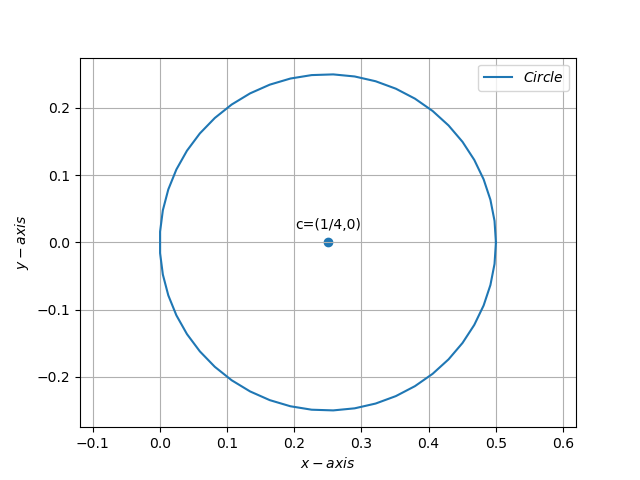
\includegraphics[width=0.75\columnwidth]{chapters/11/10/3/17/figs/fig.png}
\caption{}
\label{fig:chapters/11/10/3/17/1}
\end{figure}

\item If $p$ is the length of perpendicular from origin to the line whose intercepts on the axes are $a$ and $b$, then show that 
\begin{align}
	\frac{1}{p^2} = \frac{1}{a^2}+ \frac{1}{b^2}
\label{eq:11/10/3/18}
\end{align}
\label{chapters/11/10/3/18}
\\
\solution
\iffalse
\documentclass[journal,12pt,twocolumn]{IEEEtran}
%
\usepackage{setspace}
\usepackage{gensymb}
%\doublespacing
\singlespacing

%\usepackage{graphicx}
%\usepackage{amssymb}
%\usepackage{relsize}
\usepackage[cmex10]{amsmath}
%\usepackage{amsthm}
%\interdisplaylinepenalty=2500
%\savesymbol{iint}
%\usepackage{txfonts}
%\restoresymbol{TXF}{iint}
%\usepackage{wasysym}
\usepackage{amsthm}
%\usepackage{iithtlc}
\usepackage{mathrsfs}
\usepackage{txfonts}
\usepackage{stfloats}
\usepackage{bm}
\usepackage{cite}
\usepackage{cases}
\usepackage{subfig}
%\usepackage{xtab}
\usepackage{longtable}
\usepackage{multirow}
%\usepackage{algorithm}
%\usepackage{algpseudocode}
\usepackage{enumitem}
\usepackage{mathtools}
\usepackage{steinmetz}
\usepackage{tikz}
\usepackage{circuitikz}
\usepackage{verbatim}
\usepackage{tfrupee}
\usepackage[breaklinks=true]{hyperref}
%\usepackage{stmaryrd}
\usepackage{tkz-euclide} % loads  TikZ and tkz-base
%\usetkzobj{all}
\usetikzlibrary{calc,math}
\usepackage{listings}
    \usepackage{color}                                            %%
    \usepackage{array}                                            %%
    \usepackage{longtable}                                        %%
    \usepackage{calc}                                             %%
    \usepackage{multirow}                                         %%
    \usepackage{hhline}                                           %%
    \usepackage{ifthen}                                           %%
  %optionally (for landscape tables embedded in another document): %%
    \usepackage{lscape}     
\usepackage{multicol}
\usepackage{chngcntr}
%\usepackage{enumerate}
\usepackage{graphicx}
%\usepackage{wasysym}
%\newcounter{MYtempeqncnt}
\DeclareMathOperator*{\Res}{Res}
%\renewcommand{\baselinestretch}{2}
\renewcommand\thesection{\arabic{section}}
\renewcommand\thesubsection{\thesection.\arabic{subsection}}
\renewcommand\thesubsubsection{\thesubsection.\arabic{subsubsection}}

\renewcommand\thesectiondis{\arabic{section}}
\renewcommand\thesubsectiondis{\thesectiondis.\arabic{subsection}}
\renewcommand\thesubsubsectiondis{\thesubsectiondis.\arabic{subsubsection}}

% correct bad hyphenation here
\hyphenation{op-tical net-works semi-conduc-tor}
\def\inputGnumericTable{}                                 %%

\lstset{
%language=C,
frame=single, 
breaklines=true,
columns=fullflexible
}
%\lstset{
%language=tex,
%frame=single, 
%breaklines=true
%}

\begin{document}
%


\newtheorem{theorem}{Theorem}[section]
\newtheorem{problem}{Problem}
\newtheorem{proposition}{Proposition}[section]
\newtheorem{lemma}{Lemma}[section]
\newtheorem{corollary}[theorem]{Corollary}
\newtheorem{example}{Example}[section]
\newtheorem{definition}[problem]{Definition}
%\newtheorem{thm}{Theorem}[section] 
%\newtheorem{defn}[thm]{Definition}
%\newtheorem{algorithm}{Algorithm}[section]
%\newtheorem{cor}{Corollary}
\newcommand{\BEQA}{\begin{eqnarray}}
\newcommand{\EEQA}{\end{eqnarray}}
\newcommand{\define}{\stackrel{\triangle}{=}}

\bibliographystyle{IEEEtran}
%\bibliographystyle{ieeetr}


\providecommand{\mbf}{\mathbf}
\providecommand{\pr}[1]{\ensuremath{\Pr\left(#1\right)}}
\providecommand{\qfunc}[1]{\ensuremath{Q\left(#1\right)}}
\providecommand{\sbrak}[1]{\ensuremath{{}\left[#1\right]}}
\providecommand{\lsbrak}[1]{\ensuremath{{}\left[#1\right.}}
\providecommand{\rsbrak}[1]{\ensuremath{{}\left.#1\right]}}
\providecommand{\brak}[1]{\ensuremath{\left(#1\right)}}
\providecommand{\lbrak}[1]{\ensuremath{\left(#1\right.}}
\providecommand{\rbrak}[1]{\ensuremath{\left.#1\right)}}
\providecommand{\cbrak}[1]{\ensuremath{\left\{#1\right\}}}
\providecommand{\lcbrak}[1]{\ensuremath{\left\{#1\right.}}
\providecommand{\rcbrak}[1]{\ensuremath{\left.#1\right\}}}
\theoremstyle{remark}
\newtheorem{rem}{Remark}
\newcommand{\sgn}{\mathop{\mathrm{sgn}}}
\providecommand{\abs}[1]{\left\vert#1\right\vert}
\providecommand{\res}[1]{\Res\displaylimits_{#1}} 
\providecommand{\norm}[1]{\left\lVert#1\right\rVert}
%\providecommand{\norm}[1]{\lVert#1\rVert}
\providecommand{\mtx}[1]{\mathbf{#1}}
\providecommand{\mean}[1]{E\left[ #1 \right]}
\providecommand{\fourier}{\overset{\mathcal{F}}{ \rightleftharpoons}}
%\providecommand{\hilbert}{\overset{\mathcal{H}}{ \rightleftharpoons}}
\providecommand{\system}{\overset{\mathcal{H}}{ \longleftrightarrow}}
	%\newcommand{\solution}[2]{\textbf{Solution:}{#1}}
\newcommand{\solution}{\noindent \textbf{Solution: }}
\newcommand{\cosec}{\,\text{cosec}\,}
\providecommand{\dec}[2]{\ensuremath{\overset{#1}{\underset{#2}{\gtrless}}}}
\newcommand{\myvec}[1]{\ensuremath{\begin{pmatrix}#1\end{pmatrix}}}
\newcommand{\mydet}[1]{\ensuremath{\begin{vmatrix}#1\end{vmatrix}}}
%\numberwithin{equation}{section}
\numberwithin{equation}{subsection}
%\numberwithin{problem}{section}
%\numberwithin{definition}{section}
\makeatletter
\@addtoreset{figure}{problem}
\makeatother

\let\StandardTheFigure\thefigure
\let\vec\mathbf
%\renewcommand{\thefigure}{\theproblem.\arabic{figure}}
\renewcommand{\thefigure}{\theproblem}
%\setlist[enumerate,1]{before=\renewcommand\theequation{\theenumi.\arabic{equation}}
%\counterwithin{equation}{enumi}


%\renewcommand{\theequation}{\arabic{subsection}.\arabic{equation}}

\def\putbox#1#2#3{\makebox[0in][l]{\makebox[#1][l]{}\raisebox{\baselineskip}[0in][0in]{\raisebox{#2}[0in][0in]{#3}}}}
     \def\rightbox#1{\makebox[0in][r]{#1}}
     \def\centbox#1{\makebox[0in]{#1}}
     \def\topbox#1{\raisebox{-\baselineskip}[0in][0in]{#1}}
     \def\midbox#1{\raisebox{-0.5\baselineskip}[0in][0in]{#1}}

\vspace{3cm}


\title{Question : 11.10.3.18}
\author{Nikam Pratik Balasaheb (EE21BTECH11037)}


% make the title area
\maketitle

\newpage

%\tableofcontents

\bigskip

\renewcommand{\thefigure}{\theenumi}
\renewcommand{\thetable}{\theenumi}
%\renewcommand{\theequation}{\theenumi}

\section{Problem}

\section{Solution}
\fi
The x-intercept of the line is $\vec{A} = \myvec{a\\0}$ and the y-intercept is $\vec{B} = \myvec{0\\b}$
The direction vector of the line is given by
\begin{align}
	\vec{m} &= \myvec{a\\0} -\myvec{0\\b}\\
	&= \myvec{a\\-b}
\end{align}
The normal vector is,
\begin{align}
	\vec{n} = \myvec{b\\a}
\end{align}
The line equation is,
\begin{align}
	\vec{n}^{\top}\brak{ \vec{x} - \vec{A}} &= 0\\
\implies	\myvec{b & a}\brak{\vec{x} - \myvec{a\\0}} &= 0\\
\implies	\myvec{ b & a}\vec{x} &= ab
\end{align}
Thus,
\begin{align} 
 	c = ab
 \end{align}
and
the perpendicular distance from the origin  to the line is
\begin{align}
	p &= \frac{\abs{ \vec{n}^{\top}\vec{O} - c}}{\norm{\vec{n}}}\\
	&= \frac{ab}{\sqrt{a^2+b^2}}\\
	\implies \frac{1}{p^2} &= \frac{a^2 +b^2}{a^2b^2}\\
	&= \frac{1}{a^2}+\frac{1}{b^2}
\end{align}

\item Find the points on the x-axis, whose distances from the line $\frac{x}{3}+\frac{y}{4}=1$ are 4 units.
\label{chapters/11/10/3/5}
	\\
	\solution
\iffalse
\documentclass[12pt]{article}
\usepackage{graphicx}
\usepackage{amsmath}
\usepackage{mathtools}
\usepackage{gensymb}
\usepackage{amssymb}

\newcommand{\mydet}[1]{\ensuremath{\begin{vmatrix}#1\end{vmatrix}}}
\providecommand{\brak}[1]{\ensuremath{\left(#1\right)}}
\providecommand{\norm}[1]{\left\lVert#1\right\rVert}
\newcommand{\solution}{\noindent \textbf{Solution: }}
\newcommand{\myvec}[1]{\ensuremath{\begin{pmatrix}#1\end{pmatrix}}}
\providecommand{\abs}[1]{\left\vert#1\right\vert}	
\let\vec\mathbf

\begin{document}
\begin{center}
\textbf\large{CLASS 11 CHAPTER-11 \\ LINES}

\end{center}
\section*{Exercise 10.3}


\solution
\fi
The given line can be expressed as 
\begin{align}
	\vec{n}^{\top}\vec{x}&=c,
	\text{ where }
		\vec{n} &= \myvec{4\\3} , c = 12
\end{align}
The distance formula is given by
\begin{align}
	d = \frac{\abs{\vec{n}^\top\vec{P}-c}}{\norm{\vec{n}}}
\end{align}
Let the desired point be
\begin{align}
	\vec{P} = x\vec{e}_{1} = \myvec{x\\0}
\end{align}
Substituting the values in the distance formula, 
\begin{align}
	d &= \frac{\abs{\vec{n}^\top\vec{P}-c}}{\norm{\vec{n}}}\\
	  &= \frac{\abs{x\vec{n}^\top\vec{e}_{1}-c}}{\norm{\vec{n}}}
	  \\
	  \implies 
	\abs{x\vec{n}^\top\vec{e}_{1}-c} &= d\norm{\vec{n}}
	\\
	\text{or, }	x = \frac{\pm d\norm{\vec{n}}+c}{\vec{n}^\top\vec{e}_{1}}
\end{align}
Since 
\begin{align}
	d &= 4,
\end{align}
substituting numerical values, 
\begin{align}
	x = 8,
	 -2
\end{align}
This is verified in Fig. 
\ref{fig:11/10/3/5/Fig1}.	
\begin{figure}[!h]
	\begin{center} 
	    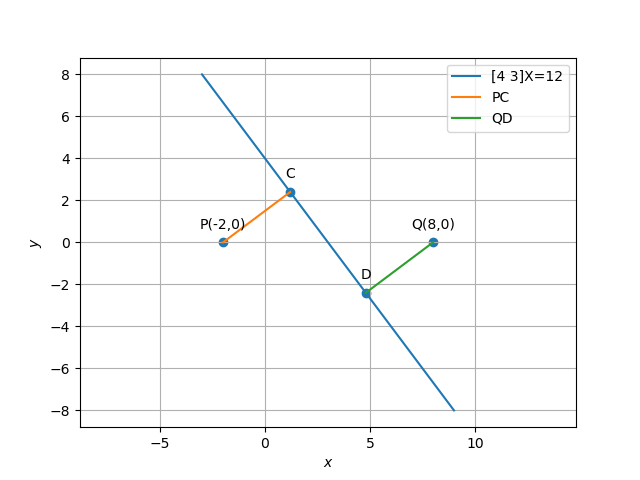
\includegraphics[width=\columnwidth]{chapters/11/10/3/5/figs/line2}
	\end{center}
\caption{}
\label{fig:11/10/3/5/Fig1}
\end{figure}



\item What are the points on the y-axis whose distance from the line $\frac{x}{3}+\frac{y}{4}=1$ is 4 units.
\\
\solution
		\iffalse
\documentclass[12pt]{article}
\usepackage{graphicx}
\usepackage[none]{hyphenat}
\usepackage{graphicx}
\usepackage{listings}
\usepackage[english]{babel}
\usepackage{graphicx}
\usepackage{caption} 
\usepackage{booktabs}
\usepackage{array}
\usepackage{amssymb} % for \because
\usepackage{amsmath}   % for having text in math mode
\usepackage{extarrows} % for Row operations arrows
\usepackage{listings}
\usepackage[utf8]{inputenc}
\lstset{
  frame=single,
  breaklines=true
}
\usepackage{hyperref}
  
%Following 2 lines were added to remove the blank page at the beginning
\usepackage{atbegshi}% http://ctan.org/pkg/atbegshi
\AtBeginDocument{\AtBeginShipoutNext{\AtBeginShipoutDiscard}}


%New macro definitions
\newcommand{\mydet}[1]{\ensuremath{\begin{vmatrix}#1\end{vmatrix}}}
\providecommand{\brak}[1]{\ensuremath{\left(#1\right)}}
\newcommand{\solution}{\noindent \textbf{Solution: }}
\newcommand{\myvec}[1]{\ensuremath{\begin{pmatrix}#1\end{pmatrix}}}
\providecommand{\norm}[1]{\left\lVert#1\right\rVert}
\providecommand{\abs}[1]{\left\vert#1\right\vert}
\let\vec\mathbf

\begin{document}

\begin{center}
\title{\textbf{LINE}}
\date{\vspace{-5ex}} %Not to print date automatically
\maketitle
\end{center}

\section{11$^{th}$ Maths - EXERCISE-10.4}
\begin{enumerate}
\end{enumerate}
\section{SOLUTION}
\fi
Given line parameters are
\begin{align}
\vec{n}=\myvec{4\\3},\,
c=12.
\end{align}
The distance of the line from y-axis
\begin{align}
d&=\frac{\vec{n}^\top\vec{P}-c}{\abs{n}}\\
\implies\pm4&=\frac{\myvec{0\\ 3y}-12}{5}\\
	\implies y&= \frac{32}{3}\text{ or }y=\frac{-8}{3}
\end{align}
See Fig. 
		\ref{fig:chapters/11/10/4/4/Figure}.
\begin{figure}[h]
\centering
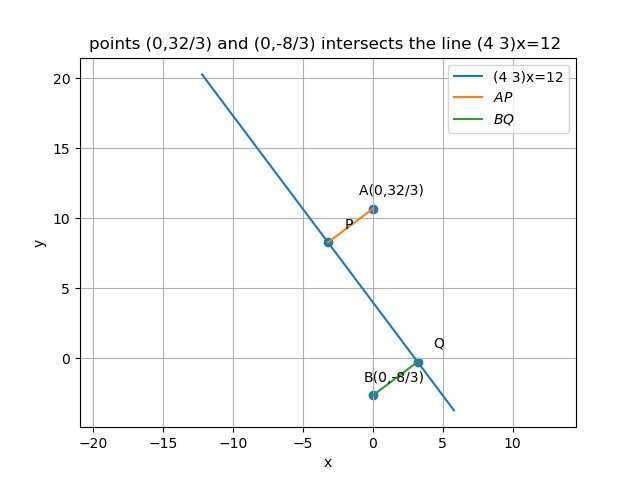
\includegraphics[width=\columnwidth]{chapters/11/10/4/4/figs/fig.png}
\caption{}
		\label{fig:chapters/11/10/4/4/Figure}
\end{figure}

\item Find perpendicular distance from the origin to the line joining the points $(\cos\theta,\sin\theta)$ and $(\cos\phi,\sin\phi)$.
\\
\solution
		The equation of the line is
\begin{align}
\myvec{\sin\phi-\sin\theta&\cos\theta-\cos\phi}\vec{x}&=\sin\brak{\phi-\theta}
\label{eq:chapters/11/10/4/5/1}
\end{align}
and from 
			\eqref{eq:PQ-final},
the distance is
\begin{align}
d
=\frac{\sin\brak{\phi-\theta}}{2\sin\brak{\frac{\phi-\theta}{2}}} = \cos\brak{\frac{\phi-\theta}{2}}
\label{eq:chapters/11/10/4/5/2}
\end{align}

\item Find the distance between parallel lines
\label{chapters/11/10/3/6}
\begin{enumerate}
	\item $15x+8y-34=0$ and  $15x+8y+31=0$ \\
	\item  $l(x+y)+p=0$ and  $l(x+y)-r=0$
\end{enumerate}
	\solution
	From \eqref{eq:parallel_lines}, the desired values are available in
  \tabref{tab:11/10/3/6}.
\begin{table}[H]
  \centering
  \begin{tabular}{|c|c|c|c|c|}
    \hline
    & $\vec{n}$ & $c_1$ & $c_2$ & $d$ \\
    \hline
    a) & $\myvec{15 \\ 8}$ & 34 & -31 & $\frac{65}{17}$ \\
    \hline
    b) & $\myvec{1 \\ 1}$ & $\frac{-p}{l}$ & $\frac{r}{l}$ & $\frac{\lvert p-r \rvert}{l\sqrt{2}}$ \\
    \hline
  \end{tabular}
  \caption{}
  \label{tab:11/10/3/6}
\end{table}

\item Find the equation of line which is equidistant from parallel lines $9x+6y-7=0$ and $3x+2y+6=0$.
\\
\solution
		\iffalse
\documentclass[journal,12pt,twocolumn]{IEEEtran}
%
\usepackage{setspace}
\usepackage{gensymb}
%\doublespacing
\singlespacing

%\usepackage{graphicx}
%\usepackage{amssymb}
%\usepackage{relsize}
\usepackage[cmex10]{amsmath}
%\usepackage{amsthm}
%\interdisplaylinepenalty=2500
%\savesymbol{iint}
%\usepackage{txfonts}
%\restoresymbol{TXF}{iint}
%\usepackage{wasysym}
\usepackage{amsthm}
%\usepackage{iithtlc}
\usepackage{mathrsfs}
\usepackage{txfonts}
\usepackage{stfloats}
\usepackage{bm}
\usepackage{cite}
\usepackage{cases}
\usepackage{subfig}
%\usepackage{xtab}
\usepackage{longtable}
\usepackage{multirow}
%\usepackage{algorithm}
%\usepackage{algpseudocode}
\usepackage{enumitem}
\usepackage{mathtools}
\usepackage{steinmetz}
\usepackage{tikz}
\usepackage{circuitikz}
\usepackage{verbatim}
\usepackage{tfrupee}
\usepackage[breaklinks=true]{hyperref}
%\usepackage{stmaryrd}
\usepackage{tkz-euclide} % loads  TikZ and tkz-base
%\usetkzobj{all}
\usetikzlibrary{calc,math}
\usepackage{listings}
    \usepackage{color}                                            %%
    \usepackage{array}                                            %%
    \usepackage{longtable}                                        %%
    \usepackage{calc}                                             %%
    \usepackage{multirow}                                         %%
    \usepackage{hhline}                                           %%
    \usepackage{ifthen}                                           %%
  %optionally (for landscape tables embedded in another document): %%
    \usepackage{lscape}     
\usepackage{multicol}
\usepackage{chngcntr}
%\usepackage{enumerate}

%\usepackage{wasysym}
%\newcounter{MYtempeqncnt}
\DeclareMathOperator*{\Res}{Res}
%\renewcommand{\baselinestretch}{2}
\renewcommand\thesection{\arabic{section}}
\renewcommand\thesubsection{\thesection.\arabic{subsection}}
\renewcommand\thesubsubsection{\thesubsection.\arabic{subsubsection}}

\renewcommand\thesectiondis{\arabic{section}}
\renewcommand\thesubsectiondis{\thesectiondis.\arabic{subsection}}
\renewcommand\thesubsubsectiondis{\thesubsectiondis.\arabic{subsubsection}}

% correct bad hyphenation here
\hyphenation{op-tical net-works semi-conduc-tor}
\def\inputGnumericTable{}                                 %%

\lstset{
%language=C,
frame=single, 
breaklines=true,
columns=fullflexible
}
%\lstset{
%language=tex,
%frame=single, 
%breaklines=true
%}


\begin{document}
%


\newtheorem{theorem}{Theorem}[section]
\newtheorem{problem}{Problem}
\newtheorem{proposition}{Proposition}[section]
\newtheorem{lemma}{Lemma}[section]
\newtheorem{corollary}[theorem]{Corollary}
\newtheorem{example}{Example}[section]
\newtheorem{definition}[problem]{Definition}
%\newtheorem{thm}{Theorem}[section] 
%\newtheorem{defn}[thm]{Definition}
%\newtheorem{algorithm}{Algorithm}[section]
%\newtheorem{cor}{Corollary}
\newcommand{\BEQA}{\begin{eqnarray}}
\newcommand{\EEQA}{\end{eqnarray}}
\newcommand{\define}{\stackrel{\triangle}{=}}

\bibliographystyle{IEEEtran}
%\bibliographystyle{ieeetr}


\providecommand{\mbf}{\mathbf}
\providecommand{\pr}[1]{\ensuremath{\Pr\left(#1\right)}}
\providecommand{\qfunc}[1]{\ensuremath{Q\left(#1\right)}}
\providecommand{\sbrak}[1]{\ensuremath{{}\left[#1\right]}}
\providecommand{\lsbrak}[1]{\ensuremath{{}\left[#1\right.}}
\providecommand{\rsbrak}[1]{\ensuremath{{}\left.#1\right]}}
\providecommand{\brak}[1]{\ensuremath{\left(#1\right)}}
\providecommand{\lbrak}[1]{\ensuremath{\left(#1\right.}}
\providecommand{\rbrak}[1]{\ensuremath{\left.#1\right)}}
\providecommand{\cbrak}[1]{\ensuremath{\left\{#1\right\}}}
\providecommand{\lcbrak}[1]{\ensuremath{\left\{#1\right.}}
\providecommand{\rcbrak}[1]{\ensuremath{\left.#1\right\}}}
\theoremstyle{remark}
\newtheorem{rem}{Remark}
\newcommand{\sgn}{\mathop{\mathrm{sgn}}}
\providecommand{\abs}[1]{\left\vert#1\right\vert}
\providecommand{\res}[1]{\Res\displaylimits_{#1}} 
\providecommand{\norm}[1]{\left\lVert#1\right\rVert}
%\providecommand{\norm}[1]{\lVert#1\rVert}
\providecommand{\mtx}[1]{\mathbf{#1}}
\providecommand{\mean}[1]{E\left[ #1 \right]}
\providecommand{\fourier}{\overset{\mathcal{F}}{ \rightleftharpoons}}
%\providecommand{\hilbert}{\overset{\mathcal{H}}{ \rightleftharpoons}}
\providecommand{\system}{\overset{\mathcal{H}}{ \longleftrightarrow}}
	%\newcommand{\solution}[2]{\textbf{Solution:}{#1}}
\newcommand{\solution}{\noindent \textbf{Solution: }}
\newcommand{\cosec}{\,\text{cosec}\,}
\providecommand{\dec}[2]{\ensuremath{\overset{#1}{\underset{#2}{\gtrless}}}}
\newcommand{\myvec}[1]{\ensuremath{\begin{pmatrix}#1\end{pmatrix}}}
\newcommand{\mydet}[1]{\ensuremath{\begin{vmatrix}#1\end{vmatrix}}}
%\numberwithin{equation}{section}
\numberwithin{equation}{subsection}
%\numberwithin{problem}{section}
%\numberwithin{definition}{section}
\makeatletter
\@addtoreset{figure}{problem}
\makeatother

\let\StandardTheFigure\thefigure
\let\vec\mathbf
%\renewcommand{\thefigure}{\theproblem.\arabic{figure}}
\renewcommand{\thefigure}{\theproblem}
%\setlist[enumerate,1]{before=\renewcommand\theequation{\theenumi.\arabic{equation}}
%\counterwithin{equation}{enumi}


%\renewcommand{\theequation}{\arabic{subsection}.\arabic{equation}}

\def\putbox#1#2#3{\makebox[0in][l]{\makebox[#1][l]{}\raisebox{\baselineskip}[0in][0in]{\raisebox{#2}[0in][0in]{#3}}}}
     \def\rightbox#1{\makebox[0in][r]{#1}}
     \def\centbox#1{\makebox[0in]{#1}}
     \def\topbox#1{\raisebox{-\baselineskip}[0in][0in]{#1}}
     \def\midbox#1{\raisebox{-0.5\baselineskip}[0in][0in]{#1}}

\vspace{3cm}


\title{Quiz 7}
\author{S Nithish}
% make the title area
\maketitle

\newpage

%\tableofcontents

\bigskip

\renewcommand{\thefigure}{\theenumi}
\renewcommand{\thetable}{\theenumi}
%\renewcommand{\theequation}{\theenumi}


\begin{abstract}
This document contains the solution of the question from NCERT 11th standard chapter 10 exercise 10.4 problem 21
\end{abstract}

%Download all python codes 
%
%\begin{lstlisting}
%svn co https://github.com/JayatiD93/trunk/My_solution_design/codes
%\end{lstlisting}

%Download all and latex-tikz codes from 
%
%\begin{lstlisting}
%svn co https://github.com/gadepall/school/trunk/ncert/geometry/figs
%\end{lstlisting}
%
\section{Exercise 10.4}
\begin{enumerate}
	\fi
The distance between  two parallel lines is given by
\begin{align}
	d = \frac{\abs{c_1-c_2}}{\norm{\vec{n}}}
\end{align}
We need to find $c$ such that,
\begin{align}
	\frac{\abs{c-c_1}}{\norm{\vec{n}}} = \frac{\abs{c-c_2}}{\norm{\vec{n}}}
\end{align}
\begin{figure}[ht]
	\centering
	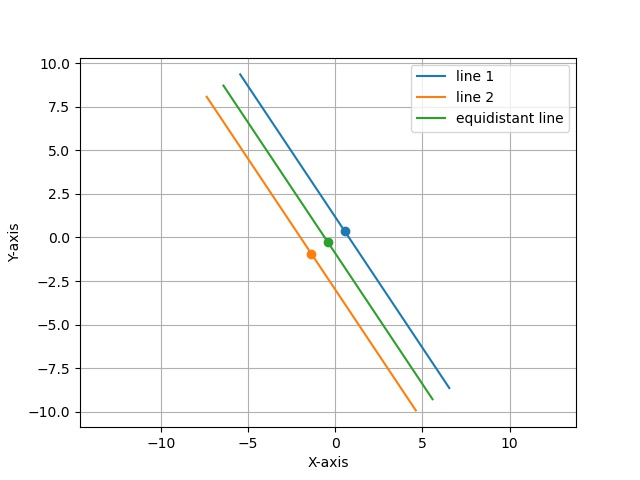
\includegraphics[width = \columnwidth]{chapters/11/10/4/21/figs/line_plot.jpg}
	\caption{}
	\label{fig:chapters/11/10/4/21/1}
\end{figure}
Since
\begin{align}
	c_1 &= \frac{7}{3},\,
c_2 = -6,\,
	\vec{n} = \myvec{3 \\ 2},
	\\
	\abs{c-\frac{7}{3}} &= \abs{c-\brak{-6}}
\implies 	c = \frac{-11}{6}
\end{align}
Hence, the desired equation is
\begin{align}
	\myvec{3 & 2}\vec{x} &= -\frac{11}{6}
\end{align}








	\item Prove that the products of the lengths of the perpendiculars drawn from the points $\myvec{\sqrt{a^2-b^2}& 0}^{\top}$ and $\myvec{-\sqrt{a^2-b^2} &0}^{\top}$ to the line $\frac{x}{a} \cos{\theta} + \frac{y}{b}\sin{\theta} =1 $ is $ b^2 $.
\\
    \solution 
		The input parameters for 
			\eqref{eq:PQ-final}
			are
\begin{align}
	\vec{n}=\myvec{\frac{\cos{\theta}}{a}  \\ \frac{\sin{\theta}}{b}},\,
  c = 1,\,
	\vec{P} =\pm \myvec{\sqrt{a^2-b^2}\\0} 
\end{align} 
The product of the distances is
\begin{align}
	d_1d_2 &=\frac{\abs{ \brak{\vec{n}^{\top} \vec{P}}^2 -  c^2 } }{\norm{\vec{n}}}
	=\frac{\abs{ \frac{\cos^2{\theta}\brak{a^2-b^2}}{a^2}- 1 }}{\frac{\cos^2{\theta}}{a^2} +\frac{\sin^2{\theta}}{b^2} }\\ 
	&= \frac{\brak{b^2 \cos^2{\theta} + a^2 \sin^2{\theta}}a^2 b^2}{\brak{b^2 \cos^2{\theta} + a^2 \sin^2{\theta}}a^2}
	= b^2
\end{align}

\item Find the equation of line  drawn perpendicular to the line $\frac{x}{4}+\frac{y}{6}=1$ through the point where it meets the y-axis \\
\solution
				The given line
parameters are
\begin{align}
		\vec{n} = \myvec{3\\2},\, c=12 ,\,
	\vec{m} =\myvec{-2 \\ 3}.
\end{align}
and the point on the y-axis is
\begin{align}
	\vec{A} =\myvec{0\\6}.
\end{align}
Thus, the equation of the desired line is 
\begin{align}
	\vec{m}^\top\brak{\vec{x}-\vec{A}}&=0\label{eq:chapters/11/10/4/7/5}
	\\
\implies
			\myvec{-2 & 3}\vec{x} &=-18
		\end{align}
		See 
  \figref{fig:chapters/11/10/4/7/Figure}.
\begin{figure}[H]
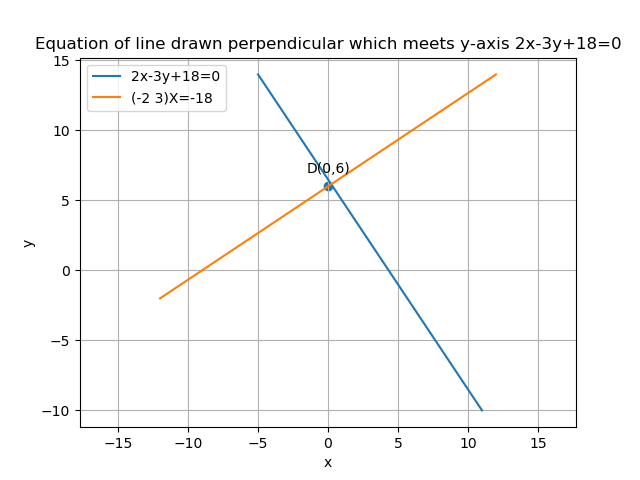
\includegraphics[width=0.75\columnwidth]{chapters/11/10/4/7/figs/fig.png}
\caption{}
  \label{fig:chapters/11/10/4/7/Figure}
\end{figure}

\item Find the equation of line whose perpendicular distance from the origin is 5 units and the angle made by the perpendicular with the positive $x$-axis is $30\degree$.
\label{chapters/11/10/2/8}
\\
\solution
			From 
\eqref{eq:chapters/11/10/2/8-final},
		Thus, the equation of lines are
\begin{align}
	\myvec{\frac{\sqrt{3}}{2}& \frac{1}{2}}\vec{x}=\pm5
\end{align}
See 
\figref{fig:chapters/11/10/2/8/Fig1}.
\begin{figure}[H]
\begin{center}
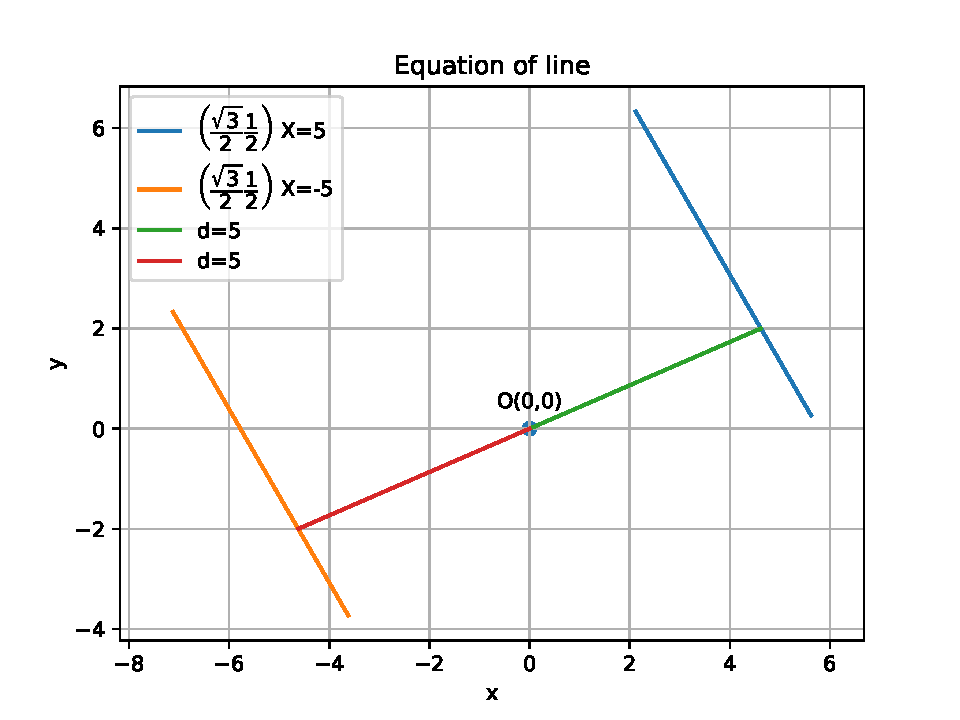
\includegraphics[width=0.75\columnwidth]{chapters/11/10/2/8/figs/fig.pdf}
\end{center}
\caption{}
\label{fig:chapters/11/10/2/8/Fig1}
\end{figure}

\item 
	Find the equation of the line passing through  (-3,5) and perpendicular to the line through the points (2,5) and (-3,6).
	\\
	\solution 
\label{chapters/11/10/2/10}
	\begin{figure}[H]
		\centering
 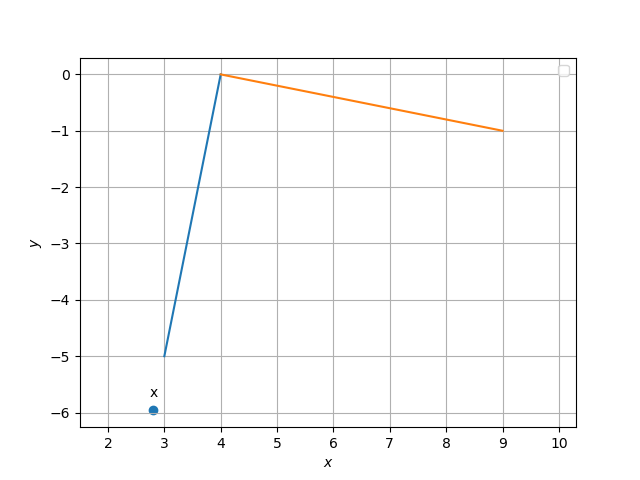
\includegraphics[width=0.75\columnwidth]{chapters/11/10/2/10/figs/Figure_1.png}
		\caption{}
		\label{fig:11/10/2/10}
  	\end{figure}
The normal vector is
\begin{align}
\vec{n} =\myvec{2 \\5} -  \myvec{-3 \\ 6} 
=\myvec{
    5\\
    -1
}
\end{align}
Thus, the equation of the line is 
\begin{align}
\myvec{
    5 &-1
	}\brak{\vec{x} - \myvec{-3 \\5}}
= 0
\\
\implies 
\myvec{
    5 &-1
	}\vec{x} 
= -20
\end{align}
See 
		\figref{fig:11/10/2/10}.

\item 
	The perpendicular from the origin to a line meets it at the point $(-2,9)$. Find the equation of the line.
\label{chapters/11/10/2/15}
	\\
	\solution
It is obvious that the normal vector to the line is 
\begin{align}
\vec{n} =\myvec{2 \\ -9} -\vec{0} 
=\myvec{2 \\ -9}
\end{align}
Hence, the equation of the line is 
\begin{align}
	\myvec{2 & -9}\brak{\vec{x} - \myvec{2 \\ -9}}&= 0
	\\
	\implies 
	\myvec{2 & -9}\vec{x} &= 85
\end{align}
See 
		\figref{fig:11/10/2/15}.
	\begin{figure}[!ht]
		\centering
 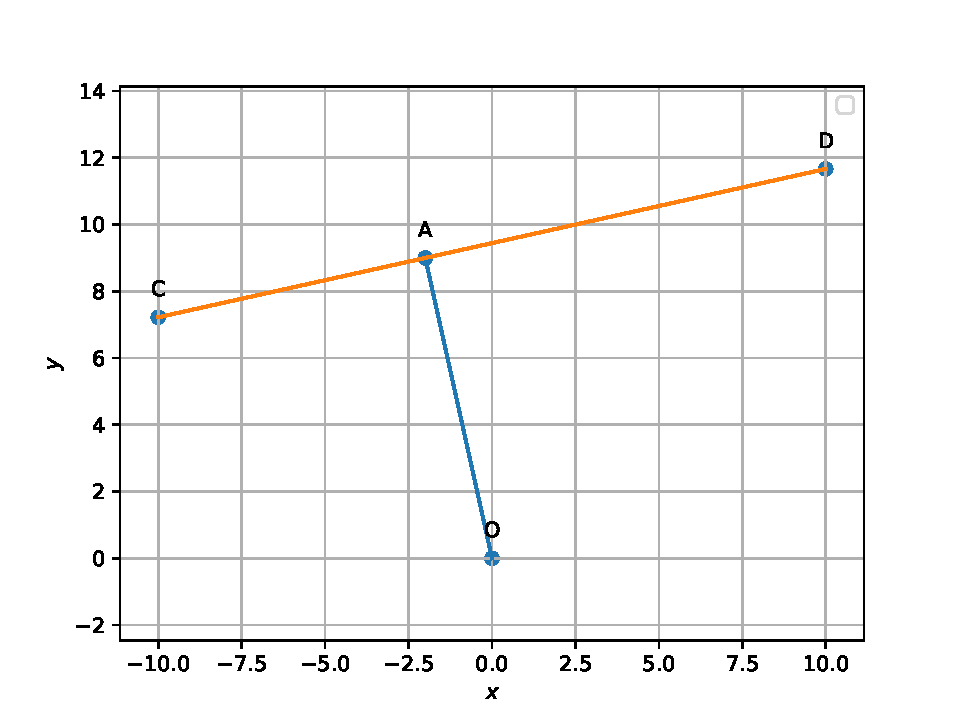
\includegraphics[width=\columnwidth]{chapters/11/10/2/15/figs/line.pdf}
		\caption{}
		\label{fig:11/10/2/15}
  	\end{figure}

\item Find the equation of line perpendicular to the line $x-7y+5=0$ and having $x$ intercept $3$\\
\label{chapters/11/10/3/8}
\solution
The desired equation is
		\begin{align}
			\myvec{7 & 1}\brak{\vec{x}-\myvec{3\\0}} &=0\\
		\implies 	\myvec{7 & 1}\vec{x} &= 21
		\end{align}
		See 
\figref{fig:chapters/11/10/3/8/Fig1}.
		\begin{figure}[!h]
\begin{center}
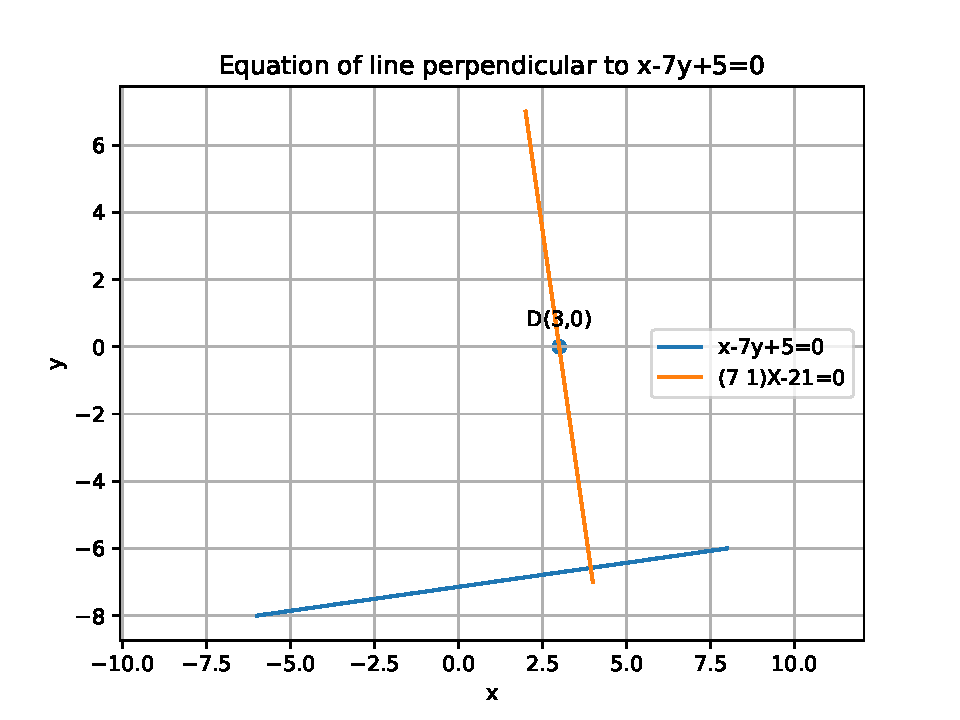
\includegraphics[width=\columnwidth]{chapters/11/10/3/8/figs/fig.pdf}
\end{center}
\caption{}
\label{fig:chapters/11/10/3/8/Fig1}
\end{figure}

	\item Find the equation of the line passing through the point $\brak{1,2,-4}$ and perpendicular to the two lines
\begin{align}
	\frac{x-8}{3}=\frac{y+19}{-16}=\frac{z-10}{7} \text{ and }\\ \frac{x-15}{3}=\frac{y-29}{8}=\frac{z-5}{-5} 
\end{align}
    \solution
		The direction vector of the desired line 
is given by 
\begin{align*}
	\myvec{3 & -16 & 7\\3 & 8 & -5}\vec{m} = 0
	\xleftrightarrow[]{R_2\leftarrow R_2-R_1}
 	\myvec{3 & -16 & 7\\0 & 24 & -12}
	\\
	\xleftrightarrow[]{R_1\leftarrow R_1+\frac{2}{3}R_2}
	\myvec{3 & 0 & -1\\0 & 24 & -12}
	\xleftrightarrow[]{R_2\leftarrow R_2/12}
	\myvec{3 & 0 & -1\\0 & 2 & -1}
\end{align*}
yielding
\begin{align}
	\vec{m} = \myvec{2\\3\\6}
\end{align}
Hence the vector equation of the line passing through $\brak{1,2,-4}$ is,
\begin{align}
	\vec{x} = \myvec{1\\2\\-4} + \kappa \myvec{2\\3\\6}
\end{align}



 \item The perpendicular from the origin to the line $y=mx+c$ meets it at the point $(-1,2)$. Find the values of m and c.
 \label{11.10.3.15}
	 \\
 \solution
 From \probref{chapters/11/10/2/15},
\begin{align}
	\vec{n} = \myvec{-1\\2} \implies m = \frac{1}{2}
\end{align}
Also, from the given equation of the line and the given point, 
\begin{align}
	c = \myvec{-m & 1}\myvec{-1\\2} = 
\frac{5}{2}  
\end{align}
\iffalse
 See \figref{fig:pic}.
\begin{figure}[H]
 \centering
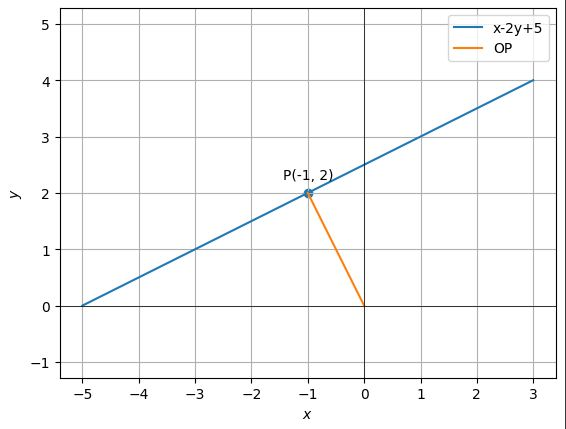
\includegraphics[width=0.75\columnwidth]{chapters/11/10/3/15/figs/graph.jpg}
 \caption{Graph}
 \label{fig:pic}
\end{figure}
\fi

\item 
A line perpendicular to the line segment joining the points $\vec{P}(1,0)$ and $\vec{Q}(2,3)$ divides it in the ratio $1:n$. Find the equation of the line.
	\\
	\solution 
\label{chapters/11/10/2/11}
\iffalse
\documentclass[journal,12pt,twocolumn]{article}
\usepackage{graphicx}
\graphicspath{{./figs/}}{}
\usepackage{amsmath,amssymb,amsfonts,amsthm}
\newcommand{\myvec}[1]{\ensuremath{\begin{pmatrix}#1\end{pmatrix}}}
\let\vec\mathbf
\title{
Matrix-Lines
}
\author{SHREYASH CHANDRA PUTTA}
\begin{document}
\maketitle
\tableofcontents

\section{Problem Statement}
\fi
A line perpendicular to the line segement joining the points (1,0) and (2,3) divides it in the ratio $1:n$. Find the equation of the line.
	\begin{figure}[!ht]
		\centering
 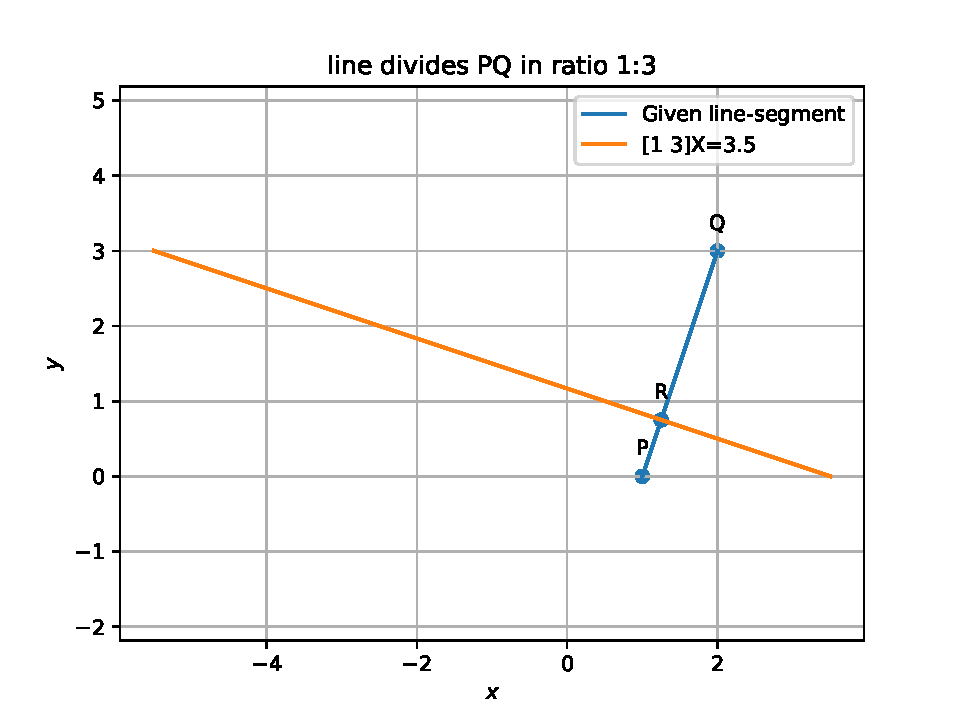
\includegraphics[width=\columnwidth]{chapters/11/10/2/11/figs/linefig.pdf}
		\caption{}
		\label{fig:11/10/2/11}
  	\end{figure}
	\\
	\solution 
\iffalse
(note: we are taking n as user Input) .

% 

\begin{table}[h]
    \centering
    \begin{tabular}{|c|c|c|}
       \hline
       \textbf{Symbol}&\textbf{Value}&\textbf{Description}  \\
       \hline
	    $\vec{P}$ & $\myvec{
		    1\\
		    0}$
	    & given point\\
        \hline
	    $\vec{Q}$ & $\myvec{2\\3}$
 & given point\\
        \hline
	    $\vec{R}$ & $\myvec{
  \frac{2+n}{1+n}\\
  \frac{3}{1+n}}$
 & intersecting point  \\
       \hline
    \end{tabular}
    \caption{Parameters}
    \label{tab:my_label}
\end{table}

%\section{Construction}

\begin{figure}[h]
    \centering
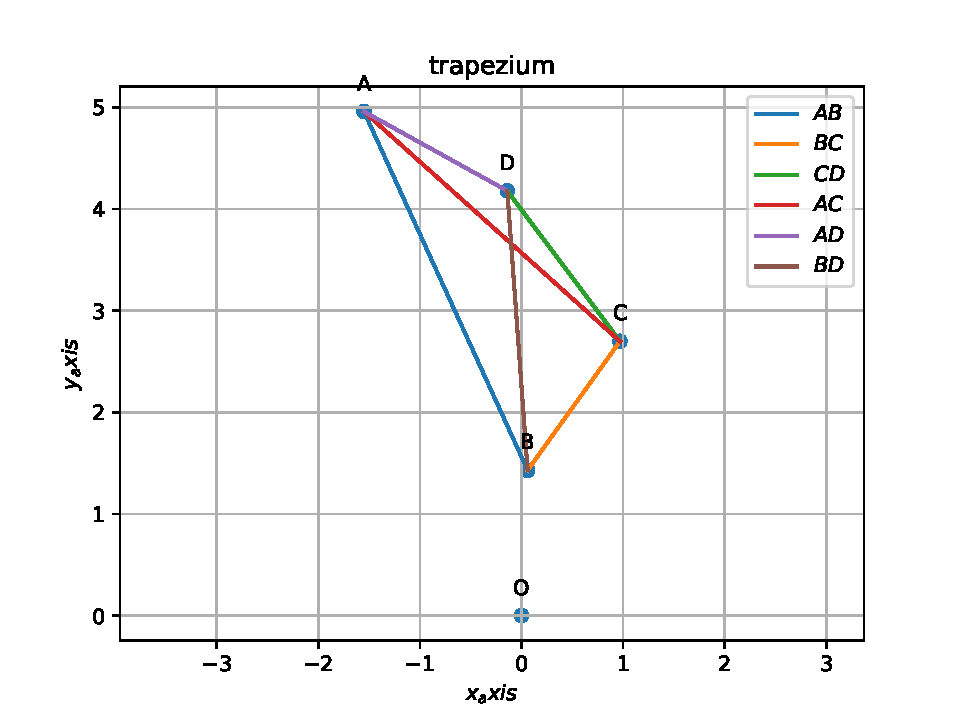
\includegraphics[width=\columnwidth]{fig/linefig.pdf}
    \caption{Equation of the required Straight Line}
    \label{fig:my_label}
\end{figure}




\section{Solution}

Given that resultant will divide the equation of line in the ratio 1:n and the line is perpendicular to line segment joining the points (1,0)and(2,3)  ) \\
%so, b = 9 - a  \\
\\
\fi 
Let 
\begin{align}
{\vec{P}}=\myvec{
  1\\
  0},
 {\vec{Q}}=\myvec{
  2\\
  3}
\end{align}
\iffalse
%	\vec{n^{\top}}
%	\myvec{
 % a\\
  %0}
  %= c \label{eq-1}
%\end{align}
\\
\fi
The direction vector of 
$PQ$ is 
\begin{align}
	\vec{m}=
     \vec{Q
 }-  \vec{P
 }
=
     \myvec{
  1\\
  3
 }
\end{align}
\iffalse
\\
We know, that position or  directional vector of points P and Q line segement used as the normal vector
\\
\\
 The general equation of the required perpendicular line is
 ${\vec{M^{\top}}\vec{X}} = c$.
 \\
 \\
 The perpendicular line cutting a line segment P and Q in ratio 1:n is passes through the point R.
 \fi
 Also, using section formula, 
 \begin{align}
	 \vec{R}=\frac{\vec{Q}+n\vec{P}}{1+n}
\end{align}
and the 
equation of line passing through ${\vec{R}}$ is
\begin{align}
	\vec{m}^{\top}\brak{\vec{x}-\vec{R}}=0
\\
\implies 
	   \myvec{
		   1 &  3}\vec{x}
	   &= \myvec{
  1\ 3}\myvec{
  \frac{2+n}{1+n}\\
  \frac{3}{1+n}} 
  \\
	&=	  \frac{11+n}{1+n} 
\end{align}
\iffalse



 
\section{Software}
Download the following code using,
\begin{table}[h]
    \centering
    \begin{tabular}{|c|}
    \hline \\
         svn co https://github.com/chanduputta/ \\FWC-Module1Assignments/blob/\\main/assignment4/line/lines3.py  \\
         \\
\hline
    \end{tabular}
\end{table}
\\
and execute the code by using command
\begin{center}
	\textbf{cmd:}
{Python3  lines3.py}\\
	\textbf{Then,}
{input your required n value}
\end{center}

\section{Conclusion}
\begin{center}
We found the equation of a line perpendicular to the line segement joining the points (1,0)and(2,3) divides it in the ratio 1:n .
\end{center}
\end{document}
\fi

\item Find the vector equation of a plane which is at a distance of 7 units from the origin and normal to the vector $3\hat{i}+5\hat{j}-6\hat{k}$.
	\\
    \solution
		\iffalse
\documentclass[12pt]{article}
\usepackage{graphicx}
\usepackage[none]{hyphenat}
\usepackage{graphicx}
\usepackage{listings}
\usepackage[english]{babel}
\usepackage{graphicx}
\usepackage{caption} 
\usepackage{booktabs}
\usepackage{array}
\usepackage{amssymb} % for \because
\usepackage{amsmath}   % for having text in math mode
\usepackage{extarrows} % for Row operations arrows
\usepackage{listings}
\lstset{
  frame=single,
  breaklines=true
}
\usepackage{hyperref}
  
%Following 2 lines were added to remove the blank page at the beginning
\usepackage{atbegshi}% http://ctan.org/pkg/atbegshi
\AtBeginDocument{\AtBeginShipoutNext{\AtBeginShipoutDiscard}}


%New macro definitions
\newcommand{\mydet}[1]{\ensuremath{\begin{vmatrix}#1\end{vmatrix}}}
\providecommand{\brak}[1]{\ensuremath{\left(#1\right)}}
\providecommand{\norm}[1]{\left\lVert#1\right\rVert}
\newcommand{\solution}{\noindent \textbf{Solution: }}
\newcommand{\myvec}[1]{\ensuremath{\begin{pmatrix}#1\end{pmatrix}}}
\providecommand{\abs}[1]{\left\vert#1\right\vert}
\let\vec\mathbf

\begin{document}

\begin{center}
\title{\textbf{Equation  of Unit Vector}}
\date{\vspace{-5ex}} %Not to print date automatically
\maketitle
\end{center}
\setcounter{page}{1}
\section{12$^{th}$ Maths - Chapter 11}
\textbf{This is Problem-2 from Exercise 3.2}
\begin{enumerate}
\section{Solution}
\fi
From the given information, 
\begin{align} 
\vec{n}=\myvec{3\\5\\-6},\,
	d=\frac{\abs{c}}{\norm{\vec{n}}} = 7
\end{align}	  
yielding
\begin{align}
c =\pm7\sqrt{70}
\end{align}	  

\item Find the equation of a plane which is at a distance 3$\sqrt{3}$ units from origin and the normal to which is equally inclined to the coordinate axis.
\item If the line drawn from the point $(-2,-1,-3)$ meets a plane at right angle at the point $(1,-3,3)$, find the equation of the plane.
\item O is the origin and A is $(a,b,c)$. Find the direction cosines of the line OA and the equation of the plane through A at right angle at OA.
\item Two systems of rectangular axis have the same origin. If a plane cuts them at distances $a,b,c$ and $a^{\prime},b^{\prime},c^{\prime}$, respectively, from the origin, prove that $$\frac{1}{a^2}+\frac{1}{b^2}+\frac{1}{c^2}=\frac{1}{{a^{\prime}}^2}+\frac{1}{{b^{\prime}}^2}+\frac{1}{{c^{\prime}}^2}$$.
\item Find the equation of the plane through the points $(2,1,-1)$ and $(-1,3,4),$ and 
perpendicular to the plane $x-2y+4z=10.$
\item If the foot of perpendicular drawn from the origin to a plane is $(5,-3,-2)$, then the equation of the plane is $\overrightarrow{r} \cdot (5\hat{i}-3\hat{j}-2\hat{k})=38.$
\item  $\vec{P}(0,2)$ is the point of intersection of $y$-axis and perpendicular bisector of line segment joining the points $\vec{A}(-1,1) \text{ and } \vec{B}(3,3)$.
	\item The distance of the point $\vec{P}(2, 3)$ from the x-axis is

\begin{enumerate}
\item 2
\item 3
\item 1
\item 5 
\end{enumerate}

\item Find the foot of perpendicular from the point $(2,3,-8)$ to the line  
\begin{align*}
	\dfrac{4-x}{2}=\dfrac{y}{6}=\dfrac{1-z}{3}.
\end{align*}
	Also, find the perpendicular distance from the given point to the line.
\item Find the distance of a point $(2,4,-1)$ from the line $$\frac{x+5}{1}=\frac{y+3}{4}=\frac{z-6}{-9}$$.
\item Find the length and the foot of perpendicular from the point $ \brak{1,\dfrac{3}{2} ,2 }$ to the plane $2x-2y+4z+5=0.$
\item Show that the points $(\hat{i}-\hat{j}+3\hat{k})$ and $3(\hat{i}+\hat{j}+\hat{k})$ are equidistant from the plane $\overrightarrow{r} \cdot (5\hat{i}+2\hat{j}-7\hat{k})+9=0$ and lie on opposite side of it.
\item The distance of the plane $\overrightarrow{r} \cdot \brak{ \dfrac{2}{7}\hat{i}+\dfrac{3}{7}\hat{j}-\dfrac{6}{7}\hat{k}}=1$ from the origin is 
\begin{enumerate}
	\item 1
	\item 7
	\item $\frac{1}{7}$
	\item None of these	
\end{enumerate}
\item Equation of the line passing through the point $(a\cos^3\theta, a\sin^3\theta)$ and perpendicular to the line $x\sec\theta+y\csc\theta=a$ is $x\cos\theta-y\sin\theta=\alpha\sin2\theta$.
\item Find the equation of the line passing through the point (5,2) and perpendicular to the line joining the points (2,3) and (3, -1).
\item Find the points on the line $x+y=4$ which lie at a unit distance from the line $4x+3y=10$.
\item Find the equation of a straight line on which length of perpendicular from the origin is four units and the line makes on angle of 120$\degree$ with the positive direction of $x$-axis. 
\item Find the equation of one of the sides of an isosceles right angled triangle whose hypotenuse is given by $3x+4y=4$ and the opposite vertex of the hypotenuse is (2,2).
\item In what direction should a line be drawn through the point (1,2) so that its point of intersection with line $x+y=4$ is at a distance $\sqrt{6}{3}$. 
\item The equation of the straight line passing through the point (3,2) and perpendicular to the line $y=x$ is
\begin{enumerate}
\item $x-y=5$
\item $x+y=5$
\item $x+y=1$
\item $x-y=1$
\end{enumerate}
\item The equation of the line passing through the point (1,2) and perpendicular to the line $x+y+1=0$ is
\begin {enumerate}
\item $y-x+1=0$
\item $y-x-1=0$
\item $y-x+2=0$
\item $y-x-1=0$
\end{enumerate}
\item The distance of the point of intersection of the lines $2x-3y+5=0 \text{ and }3x+4y=0$ from the line $5x-2y=0$ is
\begin{enumerate}
\item $\frac{130}{17\sqrt{29}}$
\item $\frac{13}{7\sqrt{29}}$
\item $\frac{130}{7}$
\item none of these
\end{enumerate}
\item The equations of the lines passing through the point (1,0) and at a distance $\frac{\sqrt{3}}{2}$ from the origin, are 
\begin{enumerate}
\item $\sqrt{3}x+y-\sqrt{3}=0$, $\sqrt{3}x-y-\sqrt{3}=0$
\item $\sqrt{3}x+y+\sqrt{3}=0$, $\sqrt{3}x-y+\sqrt{3}=0$
\item $x+\sqrt{3}y-\sqrt{3}=0$, $\sqrt{3}y-\sqrt{3}=0$
\item None of these.
\end{enumerate}
\item The distance between the lines $y=mx+c$,\text{ and }$y=mx+c^2$ is
\begin{enumerate}
\item $\frac{c_1-c_2}{\sqrt{m+1}}$
\item $\frac{\abs{c_1-c_2}}{\sqrt{1+m^2}}$
\item $\frac{c^2-c^1}{\sqrt{1+m^2}}$
\item 0
\end{enumerate}
\item The coordinates of the foot of perpendiculars from the point (2,3) on the line $y=3x+4$ is given by 
\begin{enumerate} 
\item $\frac{37}{10}$, $\frac{-1}{10}$
\item $\frac{-1}{10}$, $\frac{37}{10}$
\item $\frac{10}{37}$, -10
\item $\frac{2}{3}$, $\frac{-1}{3}$
\end{enumerate}
\item A point equidistant from the lines $4x+3y+10=0$, $5x-12y+26=0$ and $7x+24y-50=0$ is
\begin{enumerate}
\item (1,-1)
\item (1,1)
\item (0,0)
\item (0,1)
\end{enumerate}
\item A line passes through (2,2) and is perpendicular to the line $3x+y=3$. Its $y$-intercept is 
\begin{enumerate}
\item $\frac{1}{3}$
\item $\frac{2}{3}$
\item 1
\item $\frac{4}{3}$
\end{enumerate}
\item The ratio in which the line $3x+4y+2=0$ divides the distance between the lines $3x+4y+5=0$ and $3x+4y-5=0$ is
\begin{enumerate}
\item 1:2
\item 3:7
\item 2:3
\item 2:5
\end{enumerate}
\end{enumerate}
